\section{Constraining the tensor power spectrum}
The first analysis we conducted aims to show how data from a future PIXIE-like experiment can improve current constraints on the tensor-to-scalar ratio $r$. For this analysis we first produced a fiducial set of data using $\Lambda$CDM parameters with $r=0$, which corresponds to a nno-detection of spectral distortions. At this point, we run four MCMC simulations fixing all the $\Lambda$CDM parameters to the one obtained by \emph{Planck}\cite{planck2018results} and varying the tensor-to-scalar ratio at two different scales $k_1=0.02$ Mpc$^{-1}$ and $k_2=0.005$ Mpc$^{-1}$ on a flat prior between $[0,1]$. In this way, we were able to constraint directly the tensor primordial power spectrum at these two scales, which approximately sit on top of the deionization bump probed by the CMB B-modes of polarization anisotropies. To begin with, we reproduced the constraints set by BICEP/\textit{Keck} 2018 alone (red plots in Figure \ref{fig:r_const}), then we run 3 MCMC analysis combining these data with our PXIE-like experiment. In these runs we allowed for different PIXIE foreground nuisance parameters to vary to study how constraints are change assuming a perfect knowledge of the foreground. In particular, we first allowed for all the foreground parameters to vary (blue plot in Figure \ref{fig:r_const}), then we fixed them all except for the y amplitude from reionization (green plot in Figure \ref{fig:r_const}) and lastly we fixed all of them (orange plot in Figure \ref{fig:r_const}). 
\begin{figure}[t]
        \centering
        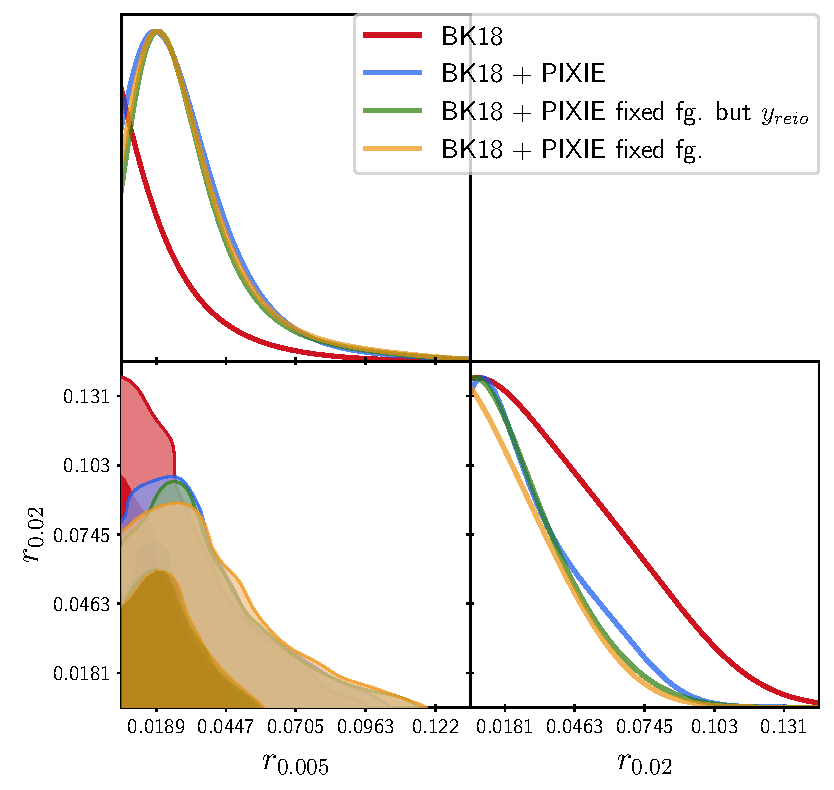
\includegraphics[width=.75\textwidth]{Constraints/BKPIXIE.pdf}
        \caption{Posterior distribution of the tensor-to-scalar ratio $r$ at two different scales $k_1=0.02$ Mpc$^{-1}$ and $k_2=0.005$ Mpc$^{-1}$. The red contour is obtained using only data from BICEP/\textit{Keck} 2018 \cite{Ade_2021} while the other contours are obtained combining BICEP/\textit{Keck} 2018 with simulated data from a PIXIE-like experiment. The blue contour is obtained by marginalizing over all the foreground/nuisance parameters, the green one by assuming a perfect knowledge of all of these parameters except $y_\text{reio}$ and the orange one including this last one.}
        \label{fig:r_const}        
    \end{figure}
Figure \ref{fig:r_const} shows how combining spectral distortions constraint with CMB anisotropies data improves the constraints on $r$ at both scales. Indeed, the 95\% CL upper limits we obtained only from BICEP/\textit{Keck} 2018 data
$$r_{0.005}<0.060,\qquad r_{0.02}<0.103,$$
once PIXIE-like data is included, get improved to 
\begin{align*}
    &r_{0.005}<0.072,\quad &r_{0.02}<0.072\qquad&\text{95\%CL with foreground,}\\
    &r_{0.005}<0.075,\quad &r_{0.02}<0.067\qquad&\text{95\%CL with only $y_{\text{reio}}$,}\\
    &r_{0.005}<0.076,\quad &r_{0.02}<0.065\qquad&\text{95\%CL with fixed foreground}.
\end{align*}
Moreover, we also translated these results into constraints on the spectral index and on the tensor to scalar ratio at a single scale $k=0.01$ Mpc$^{-1}$. 
\begin{figure}[t]
        \centering
        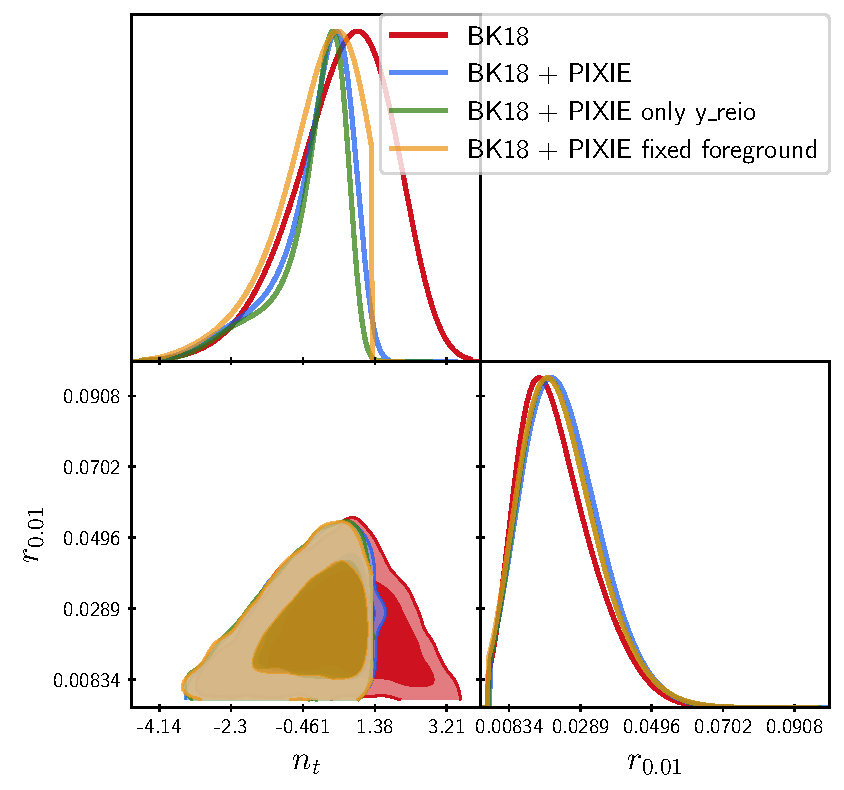
\includegraphics[width=.75\textwidth]{Constraints/nt.pdf}
        \caption{Posterior distribution of the tensor-to-scalar ratio $r$ at the scale $k=0.01$ and of the spectral index $n_t$. The red contour is obtained using only data from BICEP/\textit{Keck} 2018 \cite{Ade_2021} while the other contours are obtained combining BICEP/\textit{Keck} 2018 with simulated data from a PIXIE-like experiment. The blue contour is obtained by marginalizing over all the foreground/nuisance parameters, the green one by assuming a perfect knowledge of all of these parameters except $y_\text{reio}$ and the orange one including this last one.}
        \label{fig:nt_const}        
\end{figure}
In Figure \ref{fig:nt_const} we can appreciate how PIXIE data puts a tighter limit on the spectral index. Indeed, we found that the constraint from with BICEP/\emph{Keck} 2018 alone,
%$$r_{0.01}=0.022^{+0.008}_{-0.013} ,\qquad n_t=0.57^{+1.59}_{-0.96},\qquad \text{68\%CL}$$
$$r_{0.01}=0.022^{+0.021}_{-0.019} ,\qquad n_t=0.57^{+2.39}_{-2.66},\qquad \text{95\%CL}$$
becomes, once we introduce the PIXIE-like data,
%\begin{align*}
%    &r_{0.01}=0.024^{+0.009}_{-0.014} ,\qquad n_t=-0.13^{+1.32}_{-0.45},\quad &\text{68\%CL with foreground }\\
%    &r_{0.01}=0.024^{+0.009}_{-0.014} ,\qquad n_t=-0.22^{+1.30}_{-0.41},\quad &\text{68\%CL with only }y_\text{reio},\\
%    &r_{0.01}=0.023^{+0.009}_{-0.014} ,\qquad n_t=-0.27^{+1.34}_{-0.43},\quad &\text{68\%CL with fixed foreground. }
%\end{align*}
\begin{align*}
    &r_{0.01}=0.024^{+0.022}_{-0.021} ,\qquad &n_t=-0.13^{+1.48}_{-2.31},\quad &\text{95\%CL with foreground }\\
    &r_{0.01}=0.024^{+0.023}_{-0.021} ,\qquad &n_t=-0.22^{+1.44}_{-2.16},\quad &\text{95\%CL with only }y_\text{reio},\\
    &r_{0.01}=0.023^{+0.024}_{-0.021} ,\qquad &n_t=-0.27^{+1.52}_{-2.17},\quad &\text{95\%CL with fixed foreground. }
\end{align*}
Our analysis bends the constraints towards red tilted power spectra, narrowing the allowed window of spectral indexes. Overall, we shall note that blue spectral indexes ($n_t\sim1$) compatible with detectable tensor-induced spectral distortions, are still allowed, while far bluer spectra ($n_t\sim2$) are ruled-out. On the other hand, also the most red spectral indexes allowed by BICEP/\emph{Keck} alone ($n_t\sim-3$) are ruled-out by our PIXIE-like experiment.

We also compared the two most blue ($n_t=1.34$) and red ($n_t=-2.37$) tilted power law power spectra, allowed by the constraints we obtained. In Figure \ref{fig:analy_const_BK18} the two power spectra a shown: as we can see both power spectra lie several order of magnitude below the detection area (the area over the dashed plots) both of FIRAS and PIXIE.

Overall, we showed that spectral distortions induced by primordial gravitational waves can impact the constraint that B-modes of polarization anisotropies put on the primordial tensor power spectrum.
This strong synergy between spectral distortions and CMB anisotropies opens for the possibility of further constraining the tensor-to-scalar ratio by adding to our analysis \textit{Planck} data. 
\begin{figure}
    \centering
\begin{tikzpicture}
  \begin{axis}[
      grid=major,
      xlabel={$k$ [1/Mpc]},
      ylabel={$\mathcal{P}_T$},
      width=10cm, height=7cm,
      xmode = log, ymode = log,
      xmin = 1e-5, xmax = 1e8,
      ymin = 1e-20,
      legend pos = south east,
      legend style={font=\scriptsize},
  ]
    % Load and plot from the external file
    \addplot [thick, smooth, dashed] table {Constraints/constr_PIXIE_mu.dat};
    \addlegendentry{PIXIE analytical constraint}
    \addplot [thick, smooth, gray, dashed] table {Constraints/constr_FIRAS_mu.dat};
    \addlegendentry{FIRAS analytical constraint}
    \addplot [thick, smooth, gray] table {Constraints/Pk_blue.dat};
    \addlegendentry{BK18 + PIXIE blue $n_t$ upper limit}
    \addplot [thick, smooth, black] table {Constraints/Pk_red.dat};
    \addlegendentry{BK18 + PIXIE red $n_t$ upper limit}
  \end{axis}
\end{tikzpicture}
\caption{Comparison of the most blue tilted and red tilted power laws allowed  by the constraints set by BICEP/\emph{Keck} 2018 + PIXIE analysis (solid lines) and the analytical constraints given by PIXIE and FIRAS (dashed lines).}
\label{fig:analy_const_BK18}
\end{figure}
\section{Constraining lognormal bumps}
In this last section we discuss the second type of constraints that we obtained. We constrained the height of a lognormal bump placed at $k_\text{pk}=10$ Mpc$^{-1}$ using simulated data from the PIXIE experiment \cite{pixie}. We started producing a fiducial set of data from a power spectrum without the bump, with only the power law power spectrum which satisfies the single field inflation consistency relation $n_t=-r/8$, with $r=0.035$, and $\Lambda$CDM data obtained by the \emph{Planck} collaboration. Then using \textbf{\texttt{MontePython}} we obtained 3 different types of constraints: the first one in which we vary all the foreground parameters presented in Table \ref{tab:nui_pixie}, a second one with a fixed foreground and a last one in which, by letting vary also $y_\text{reio}$, we marginalize only over it.  In all the three cases we fixed the width of the bump at an intermediate value of $\sigma_\text{bump}=0.44$.\\
The analysis performed considering all the foreground nuisance parameters, shown in Figure \ref{fig:LN}, results in a constraint on the amplitude of the bump of $\mathcal{A}_\text{bump}<3.2\times10^{-2}$ at 95\% CL. This constraint becomes more stringent if we assume a perfect knowledge of the foreground parameters, as shown in Figure \ref{fig:LN_NN}, resulting in $\mathcal{A}_\text{bump}<7.7\times10^{-5}$. A milder constraint results instead if we marginalize only over $y_\text{reio}$, as shown in Figure \ref{fig:LN_NN_reio}, resulting in $\mathcal{A}_\text{bump}<4.0\times10^{-4}$.\\ 
\begin{figure}
    \centering
    \begin{subfigure}{0.49\textwidth}
        \centering
        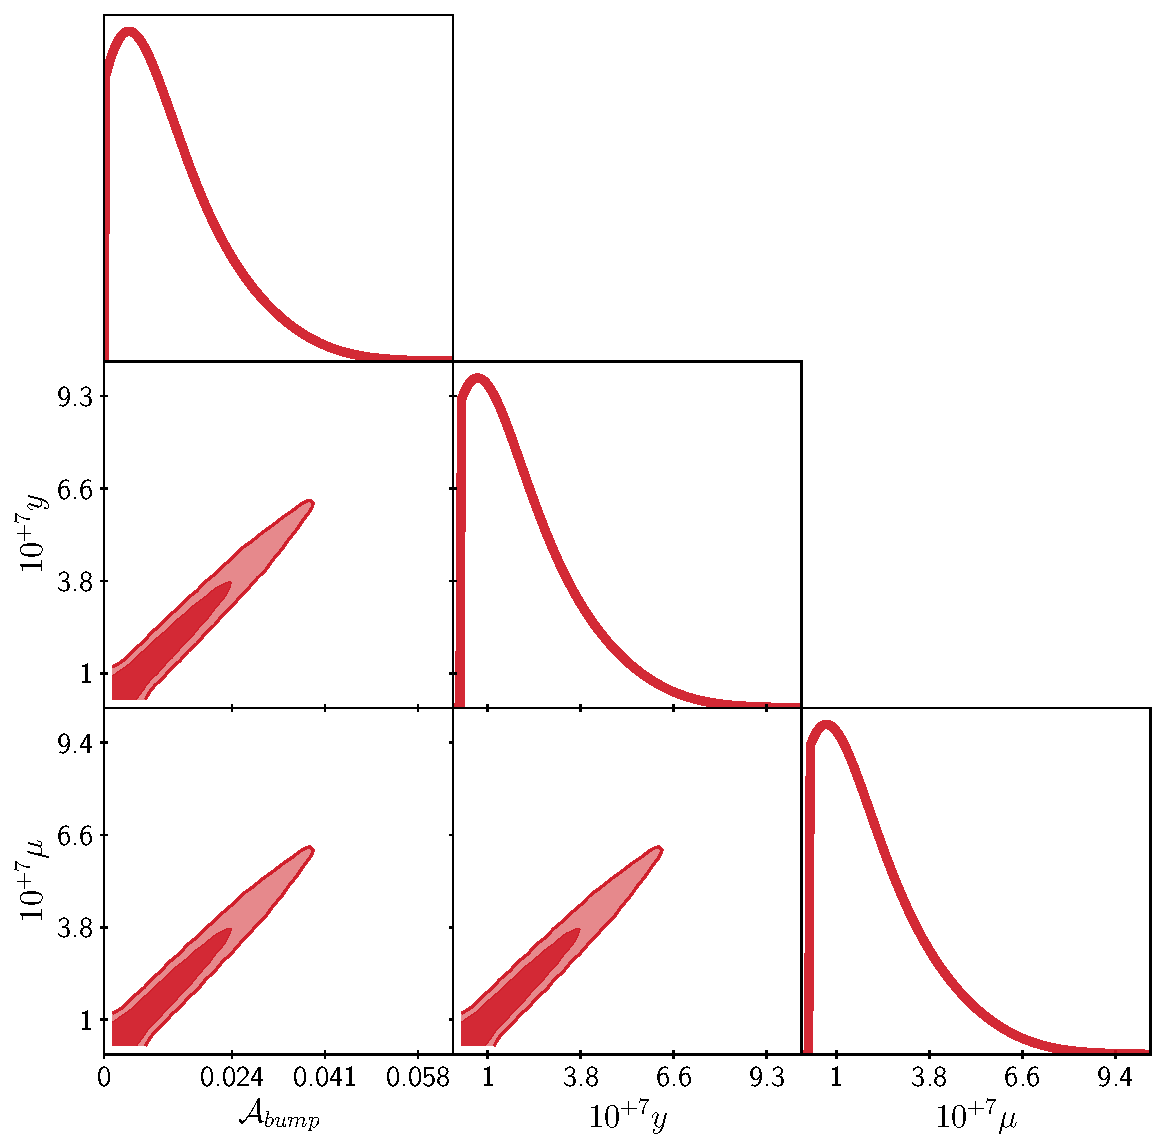
\includegraphics[width=1\textwidth]{Constraints/Lognormal.pdf}
        \caption{PIXIE with foreground}
        \label{fig:LN}        
    \end{subfigure}
    \hfill
    \begin{subfigure}{0.49\textwidth}
        \centering
        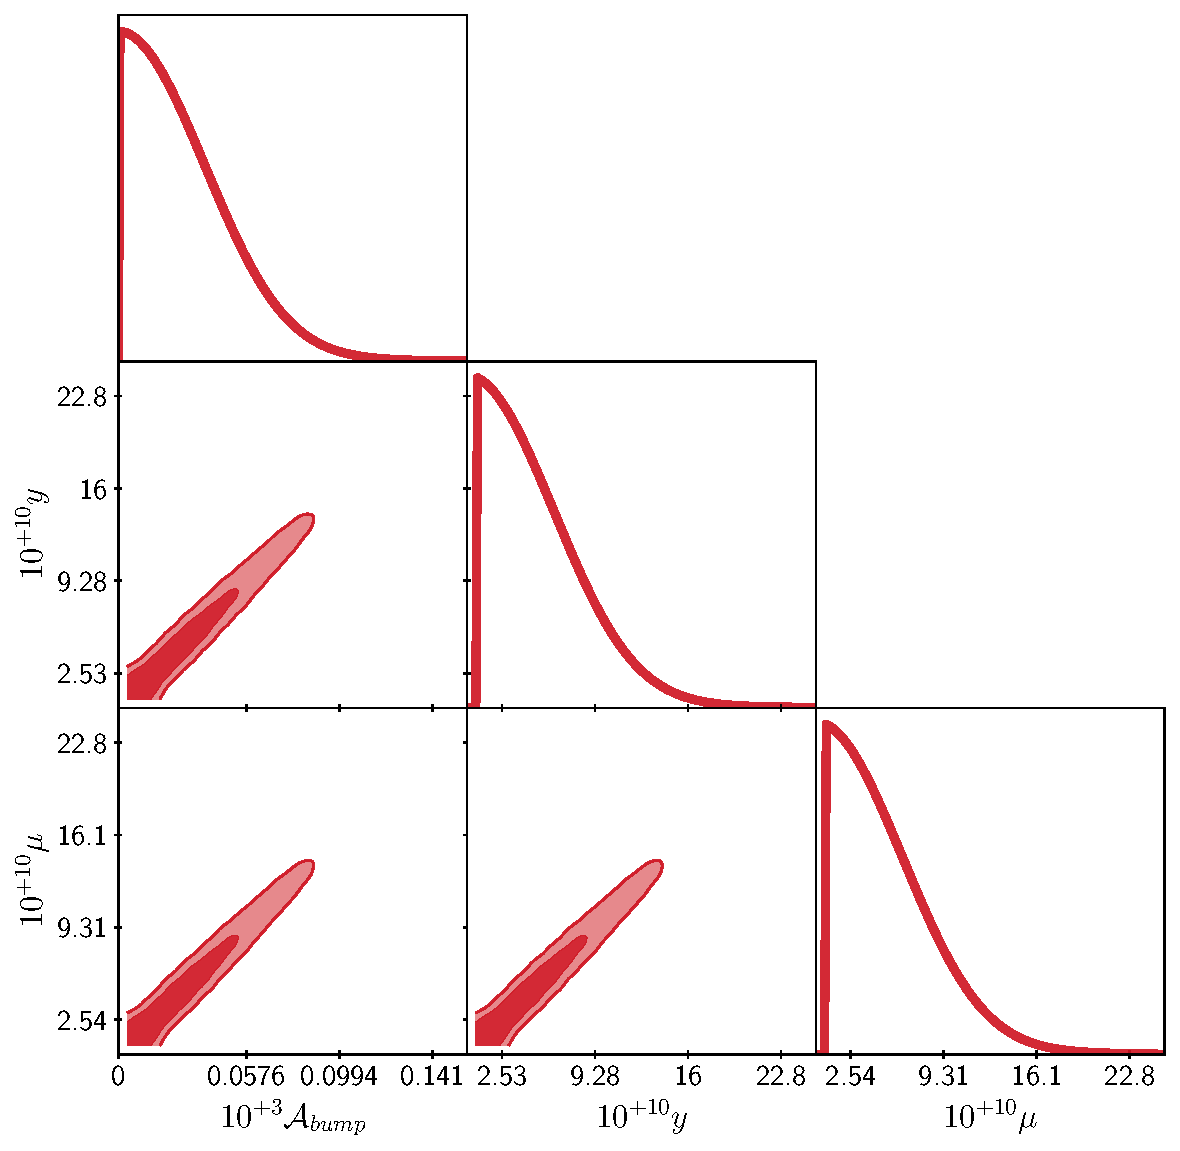
\includegraphics[width=1\textwidth]{Constraints/LN_NN.pdf}
        \caption{PIXIE without foreground}
        \label{fig:LN_NN}        
    \end{subfigure}

    \vspace{1em}

    \begin{subfigure}{0.5\textheight}
        \centering
        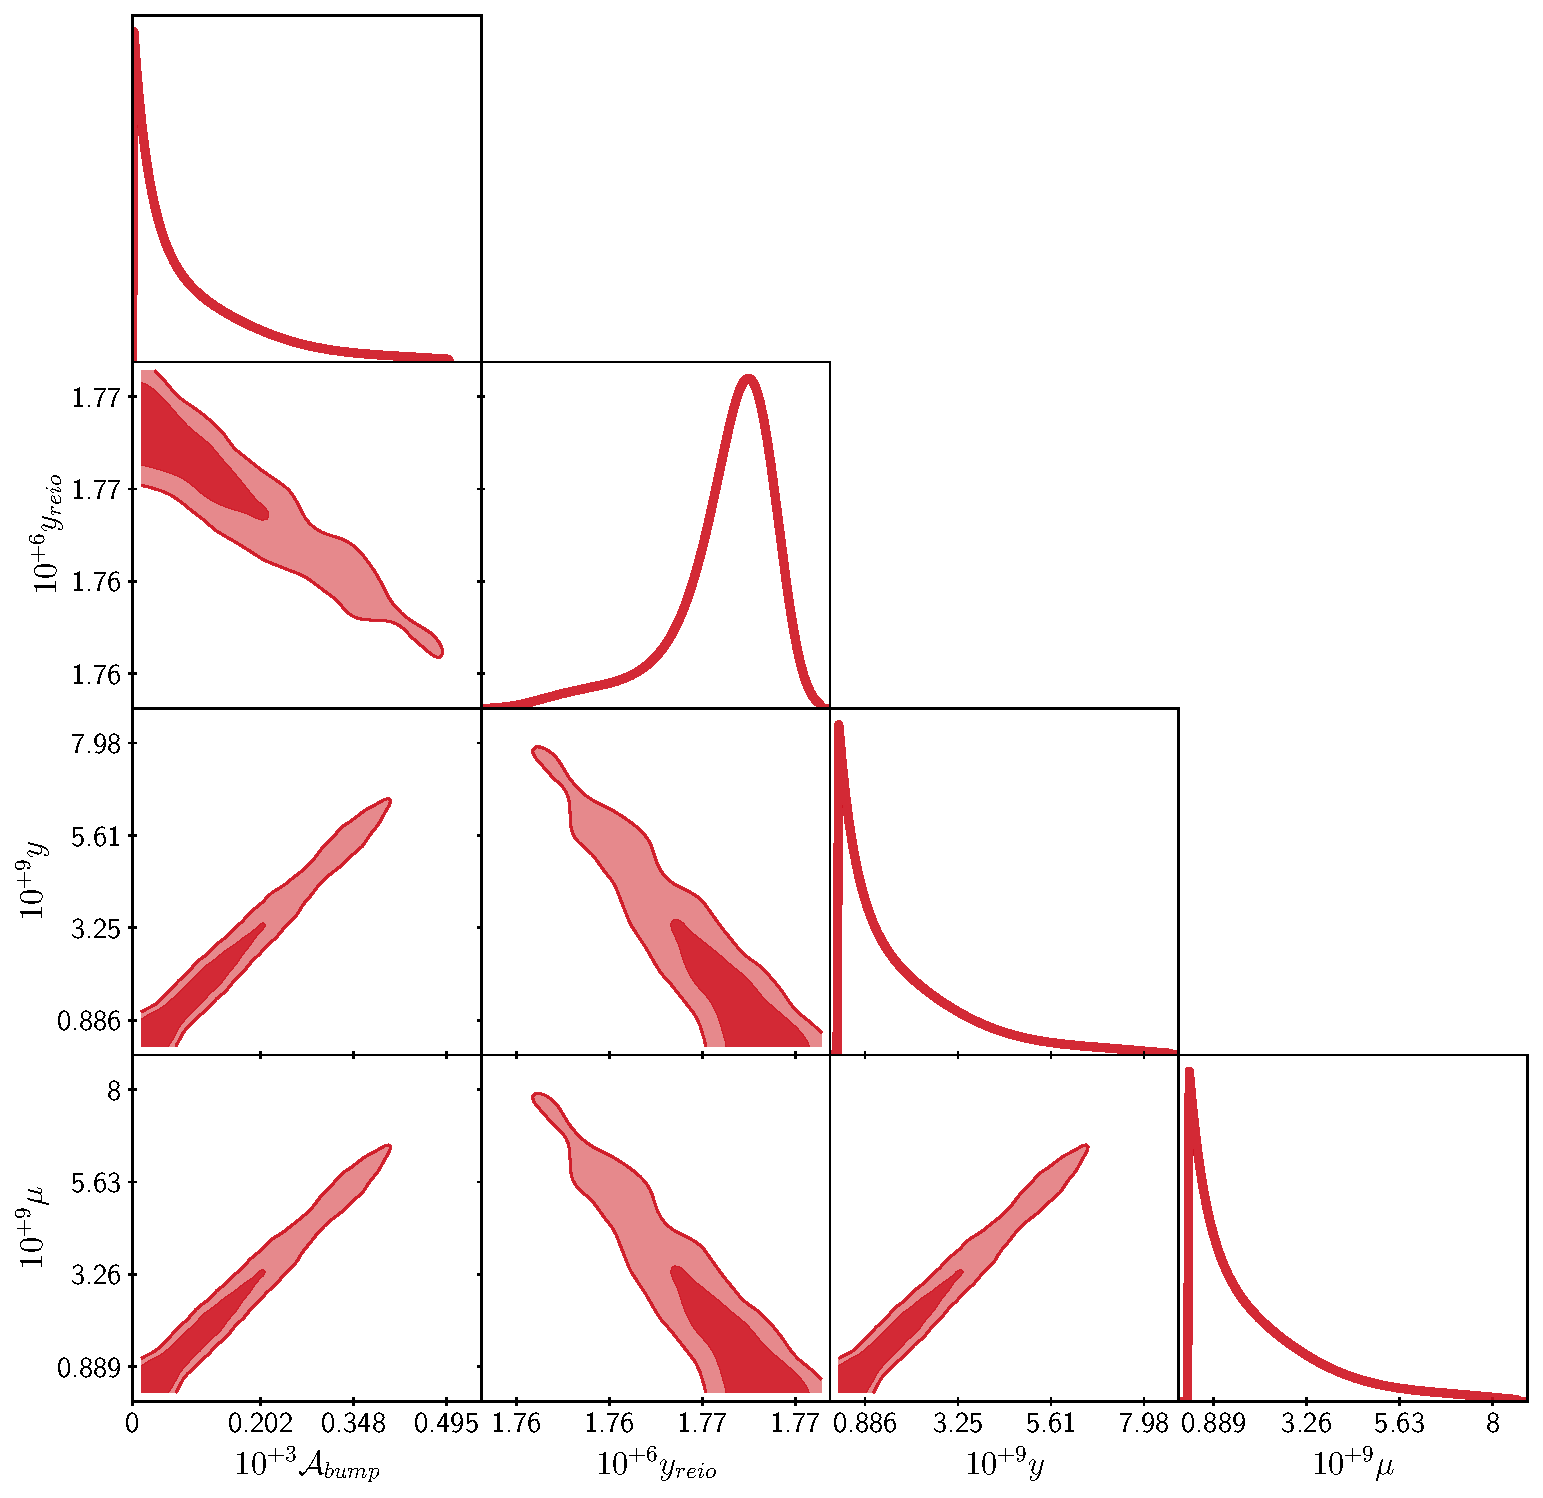
\includegraphics[width=1\textwidth]{Constraints/LN_NN_reio.pdf}
        \caption{PIXIE with only $y_\text{reio}$}
        \label{fig:LN_NN_reio}        
    \end{subfigure}
    \caption{Marginalized posterior distributions for the amplitude of a lognormal bump placed at $k_\text{pk}=10$ Mpc$^{-1}$ with width $\sigma_\text{bump}=0.44$. The three panels show the results obtained with different assumptions on the nuisance parameters.}
    \label{fig:LN_all}
\end{figure}

\begin{figure}
    \centering
\begin{tikzpicture}
  \begin{axis}[
      grid=major,
      xlabel={$k$ [1/Mpc]},
      ylabel={$\mathcal{P}_T$},
      width=12cm, height=8cm,
      xmode = log, ymode = log,
      xmin = 1e-2, xmax = 1e8,
      ymin = 1e-11, ymax = 1e3,
      legend pos = south east,
      legend style={font=\scriptsize},
  ]
    % Load and plot from the external file
    \addplot [thick, smooth, dashed] table {Constraints/constr_PIXIE_mu.dat};
    \addlegendentry{PIXIE analytical constraint}
    \addplot [thick, smooth, gray, dashed] table {Constraints/constr_FIRAS_mu.dat};
    \addlegendentry{FIRAS analytical constraint}
    \addplot [thick, smooth, black] table {Constraints/bump.dat};
    \addlegendentry{Power law + bump}
    \addplot [thick, smooth ,gray] table {Constraints/bump_reio.dat};
    \addlegendentry{Power law + bump only $y_{reio}$}
    \addplot [thick, smooth, dotted, gray] table {Constraints/bump_NN.dat};
    \addlegendentry{Power law + bump fixed foregorund}
  \end{axis}
\end{tikzpicture}
\caption{Comparison of the largest bumps allowed by our PIXIE-like analysis and the analytical constraints given by PIXIE and FIRAS (dashed lines).}
\label{fig:analy_const_bump}
\end{figure}



